% !TEX program = xelatex
\documentclass[aspectratio=169,10pt]{beamer}

%% ---------- Fonts (XeLaTeX) ----------
\usepackage{fontspec}
\setmainfont{Liberation Sans}
\setsansfont{Liberation Sans}
\setmonofont{Liberation Mono}

\usepackage[table]{xcolor}
\usepackage{tikz}
\usetikzlibrary{arrows.meta,positioning,shapes.geometric,shapes.multipart,fit,calc,backgrounds}
\usepackage{listings}
\usepackage{booktabs,array,graphicx}
\hypersetup{hidelinks}

%% ---------- Bảng màu sáng (chỉ dùng cho hình / trang trí) ----------
\definecolor{cRed}{HTML}{FF8A80}
\definecolor{cOrange}{HTML}{FFB74D}
\definecolor{cYellow}{HTML}{FFE57F}
\definecolor{cGreen}{HTML}{8EE6A0}
\definecolor{cBlue}{HTML}{81D4FA}
\definecolor{cPurple}{HTML}{CE93D8}
\definecolor{cHead}{HTML}{4D9DE0}
\arrayrulecolor{black!60}

%% ---------- Toàn bộ chữ màu đen ----------
\setbeamercolor{normal text}{fg=black,bg=white}
\setbeamercolor{structure}{fg=black}
\setbeamercolor{frametitle}{fg=black,bg=white}
\setbeamercolor{title}{fg=black}
\setbeamercolor{subtitle}{fg=black}
\setbeamercolor{item}{fg=black}
\setbeamercolor{subitem}{fg=black}
\setbeamercolor{section in toc}{fg=black}
\setbeamercolor{subsection in toc}{fg=black}
\setbeamercolor{url}{fg=black}
\setbeamercolor{alerted text}{fg=black}
\setbeamerfont{frametitle}{series=\bfseries,size=\Large}
\setbeamerfont{alerted text}{series=\bfseries}
\setbeamertemplate{navigation symbols}{}
\setbeamersize{text margin left=0.7cm,text margin right=0.7cm}
\setbeamertemplate{itemize item}{\textbullet}
\setbeamertemplate{itemize subitem}{--}
\setbeamertemplate{enumerate item}{\insertenumlabel.}
\setbeamertemplate{section in toc}{\leavevmode\textbf{\inserttocsectionnumber.}~\textbf{\inserttocsection}\par}
\setbeamertemplate{subsection in toc}{\leavevmode\hspace{1.5em}\inserttocsectionnumber.\inserttocsubsectionnumber~\inserttocsubsection\par}

\setbeamertemplate{frametitle}{%
  \vspace{5pt}{\usebeamerfont{frametitle}\insertframetitle}\par\vspace{1pt}
}
\setbeamertemplate{footline}{%
  \hbox to\paperwidth{\hspace{0.7cm}\scriptsize\textbf{Responsive \& Adaptive UI trong Flutter}\hfill\scriptsize\insertframenumber\,/\,\inserttotalframenumber\hspace{0.7cm}}\vskip5pt}

%% ---------- Macros ----------
\newcommand{\api}[1]{\texttt{\bfseries #1}}   % tên API in đậm, font mono
\newcommand{\cd}[1]{\texttt{#1}}              % code thường
\setlength{\parskip}{0pt}

%% ---------- Listings (Dart) ----------
\lstdefinelanguage{Dart}{
  morekeywords={abstract,as,async,await,break,case,catch,class,const,continue,default,do,else,enum,extends,final,finally,for,if,implements,import,in,is,late,new,null,override,return,static,super,switch,this,throw,try,var,void,while,yield,Future,Stream,StreamController,StreamBuilder,StreamSubscription,Timer,required},
  sensitive=true,
  morecomment=[l]{//},
  morestring=[b]',
  morestring=[b]"
}
\lstset{
  language=Dart,
  basicstyle=\ttfamily\scriptsize,
  keywordstyle=\bfseries,
  commentstyle=\itshape,
  stringstyle=\relax,
  frame=single,
  rulecolor=\color{black!45},
  backgroundcolor=\color{black!4},
  showstringspaces=false,
  columns=fullflexible,
  escapeinside={(*@}{@*)},
  keepspaces=true,
  xleftmargin=3pt, xrightmargin=3pt,
  aboveskip=2pt, belowskip=2pt
}

%% ---------- TikZ styles ----------
\tikzset{
  base/.style={draw=black!75, thick, rounded corners=2.5pt, align=center, text=black,
               inner sep=3.5pt, minimum height=0.8cm, font=\footnotesize},
  fr/.style={fill=cRed}, fo/.style={fill=cOrange}, fy/.style={fill=cYellow},
  fg/.style={fill=cGreen}, fb/.style={fill=cBlue}, fp/.style={fill=cPurple},
  arr/.style={-{Stealth[length=2.4mm,width=1.9mm]}, thick, black!85},
  darr/.style={-{Stealth[length=2.4mm,width=1.9mm]}, thick, black!85, dashed},
  lbl/.style={font=\scriptsize, text=black, inner sep=1.2pt},
  dot/.style={circle, fill=black, inner sep=2.2pt},
}
\newcommand{\seqlen}{4.9}
\newcommand{\seqpart}[4]{% id, x, colorstyle, label
  \node[base,#3,minimum width=2.7cm,minimum height=0.75cm] (#1) at (#2,0) {#4};
  \draw[dashed,black!45] (#1.south) -- (#2,-\seqlen);}
\newcommand{\smsg}[4]{\draw[arr] (#1,#3) -- (#2,#3) node[midway,above,lbl]{#4};}
\newcommand{\sret}[4]{\draw[darr] (#1,#3) -- (#2,#3) node[midway,above,lbl]{#4};}

\begin{document}

%% =====================================================================
%% TRANG BÌA
%% =====================================================================
\begin{frame}[plain]
  \centering
  \vspace{0.2cm}
  {\large\bfseries TRƯỜNG ĐẠI HỌC BÁCH KHOA -- ĐẠI HỌC ĐÀ NẴNG}\\[3pt]
  {\large\bfseries KHOA ĐIỆN TỬ VÀ TRÍ TUỆ NHÂN TẠO}\\[22pt]
  {\normalsize\bfseries ĐỀ TÀI}\\[5pt]
  {\LARGE\bfseries Thiết kế giao diện đa màn hình:\\ Responsive \& Adaptive UI trong Flutter}\\[14pt]
  \begin{tabular}{rl}
    \textbf{Sinh viên thực hiện:} & \textbf{Phan Văn Trà}\\
                                  & \textbf{Trần Đăng Duy}\\[4pt]
    \textbf{Giảng viên hướng dẫn:} & \textbf{TS. Nguyễn Duy Nhật Viễn}
  \end{tabular}\\[14pt]
  {\normalsize Đà Nẵng, ngày 26 tháng 11 năm 2026}
\end{frame}

\begin{frame}{Mục lục}
  \vspace{6pt}
  \large
  \tableofcontents[subsubsectionstyle=hide]
\end{frame}

%% =====================================================================
%% PHẦN 1
%% =====================================================================
\section{Cơ sở lý thuyết}
\subsection{Khái niệm Responsive và Adaptive}

\begin{frame}{1.1 \textbf{Responsive} và \textbf{Adaptive}: hai cách thích ứng giao diện}
  \footnotesize
  \renewcommand{\arraystretch}{1.45}
  \centering
  \begin{tabular}{@{}>{\raggedright\arraybackslash}p{2.2cm}>{\raggedright\arraybackslash}p{5.2cm}>{\raggedright\arraybackslash}p{5.2cm}@{}}
    \hline
    \rowcolor{cHead}\textbf{Tiêu chí} & \textbf{Responsive} & \textbf{Adaptive}\\ \hline
    \textbf{Ý tưởng} & Bố cục \textbf{co giãn liên tục} theo không gian khả dụng & \textbf{Chọn} một trong nhiều bố cục riêng theo điều kiện\\ \hline
    \textbf{Công cụ} & \api{Expanded}, \api{Flexible}, \api{GridView}, \api{ConstrainedBox} & \api{LayoutBuilder} / \api{MediaQuery} + \textbf{breakpoint}, trả về widget khác nhau\\ \hline
    \textbf{Ví dụ} & Lưới thẻ tự chia \textbf{1 $\rightarrow$ 2 $\rightarrow$ 3 cột} & Danh sách (mobile) $\leftrightarrow$ \textbf{Master--Detail} (tablet)\\ \hline
    \textbf{Phù hợp khi} & Kích thước thay đổi liên tục (kéo cửa sổ, xoay màn hình) & Cấu trúc giao diện hoặc cách tương tác khác nhau giữa các nhóm màn hình\\ \hline
  \end{tabular}

  \vspace{8pt}
  \small Thực tế thường \textbf{kết hợp cả hai}: \textbf{adaptive} chọn bố cục khung, \textbf{responsive} co giãn nội dung bên trong.
\end{frame}

\begin{frame}{1.1 Minh hoạ trực quan: \textbf{Responsive} vs \textbf{Adaptive}}
  \centering
  \begin{tikzpicture}[
    fr0/.style={draw=black!75,thick,rounded corners=3pt,fill=white},
    card/.style={draw=black!70,fill=cBlue,rounded corners=1.5pt,thick},
    det/.style={draw=black!70,fill=cGreen,rounded corners=1.5pt,thick}]
    % ---- Responsive row
    \draw[fr0] (0,0) rectangle (1.5,2.3);
    \foreach \y in {1.65,1.05,0.45}{\draw[card] (0.15,\y) rectangle (1.35,\y+0.45);}
    \draw[fr0] (2.1,0) rectangle (4.6,2.3);
    \foreach \y in {1.65,1.05,0.45}{\draw[card] (2.25,\y) rectangle (3.3,\y+0.45); \draw[card] (3.4,\y) rectangle (4.45,\y+0.45);}
    \draw[fr0] (5.2,0) rectangle (9.1,2.3);
    \foreach \y in {1.65,1.05,0.45}{\foreach \x in {5.35,6.65,7.95}{\draw[card] (\x,\y) rectangle (\x+1.15,\y+0.45);}}
    \node[font=\scriptsize] at (0.75,-0.3) {hẹp: \textbf{1 cột}};
    \node[font=\scriptsize] at (3.35,-0.3) {vừa: \textbf{2 cột}};
    \node[font=\scriptsize] at (7.15,-0.3) {rộng: \textbf{3 cột}};
    \node[align=left,anchor=west,text width=4.6cm,font=\footnotesize] at (9.5,1.15) {\textbf{Responsive}\\Cùng một cấu trúc, các phần tử \textbf{co giãn / chia lại} khi không gian đổi.};
    % ---- Adaptive row
    \begin{scope}[yshift=-3.5cm]
      \draw[fr0] (0,0) rectangle (1.5,2.3);
      \foreach \y in {1.65,1.05,0.45}{\draw[card] (0.15,\y) rectangle (1.35,\y+0.45);}
      \draw[fr0] (2.1,0) rectangle (7.1,2.3);
      \foreach \y in {1.65,1.05,0.45}{\draw[card] (2.25,\y) rectangle (3.75,\y+0.45);}
      \draw[thick,black!70] (3.95,0) -- (3.95,2.3);
      \draw[det] (4.15,0.2) rectangle (6.95,2.1);
      \foreach \y in {1.7,1.3,0.9}{\draw[black!60,thick] (4.35,\y) -- (6.7,\y);}
      \node[font=\scriptsize] at (0.75,-0.3) {\textbf{Mobile}: danh sách};
      \node[font=\scriptsize] at (4.6,-0.3) {\textbf{Tablet}: danh sách $\mid$ chi tiết};
      \node[align=left,anchor=west,text width=4.6cm,font=\footnotesize] at (9.5,1.15) {\textbf{Adaptive}\\\textbf{Đổi cấu trúc} giao diện: 1 vùng $\leftrightarrow$ 2 vùng tuỳ điều kiện hiển thị.};
    \end{scope}
  \end{tikzpicture}
\end{frame}

\subsection{MediaQuery, LayoutBuilder và breakpoint}

\begin{frame}[fragile]{1.2 \textbf{MediaQuery}: thông tin về môi trường hiển thị}
  \begin{columns}[T]
    \begin{column}{0.44\textwidth}
      \small
      \begin{itemize}\itemsep4pt
        \item \api{MediaQuery} cung cấp thông tin về \textbf{cửa sổ / màn hình} của ứng dụng.
        \item Thuộc tính hay dùng: \api{size}, \api{orientation}, \api{padding} (vùng an toàn), \api{textScaler}, \api{platformBrightness}.
        \item Dùng hàm chuyên biệt (\api{sizeOf}, \api{orientationOf}, \api{textScalerOf}) để widget \textbf{chỉ rebuild} khi đúng thuộc tính đó đổi.
        \item \textbf{Hạn chế}: cho biết kích thước \textbf{cửa sổ}, không phải vùng mà widget cha thực sự cấp cho con.
      \end{itemize}
    \end{column}
    \begin{column}{0.54\textwidth}
\begin{lstlisting}[basicstyle=\ttfamily\fontsize{6.8}{8}\selectfont]
(*@\texttt{\itshape // Kích thước cửa sổ / màn hình (dp)}@*)
final size = MediaQuery.sizeOf(context);
final width = size.width;

(*@\texttt{\itshape // Hướng màn hình}@*)
final orientation = MediaQuery.orientationOf(context);
final isLandscape =
    orientation == Orientation.landscape;

(*@\texttt{\itshape // Cỡ chữ người dùng chọn trong hệ thống}@*)
final scaler = MediaQuery.textScalerOf(context);

(*@\texttt{\itshape // Vùng an toàn (tai thỏ, thanh trạng thái)}@*)
final padding = MediaQuery.paddingOf(context);
\end{lstlisting}
    \end{column}
  \end{columns}
\end{frame}

\begin{frame}[fragile]{1.2 \textbf{LayoutBuilder}: đo không gian mà widget cha cấp}
  \begin{columns}[T]
    \begin{column}{0.40\textwidth}
      \centering
      \begin{tikzpicture}
        \node[base,fb,minimum width=3.4cm] (p) at (0,2.6) {\textbf{Widget cha}\\(Row, Expanded, pane\ldots)};
        \node[base,fg,minimum width=3.4cm] (l) at (0,0.7) {\textbf{LayoutBuilder}\\builder(context, \textbf{constraints})};
        \node[base,fo,minimum width=3.4cm] (c) at (0,-1.2) {\textbf{Widget con}\\chọn bố cục theo maxWidth};
        \draw[arr] ([xshift=-0.7cm]p.south) -- node[lbl,left]{\textbf{BoxConstraints}} ([xshift=-0.7cm]l.north);
        \draw[arr] ([xshift=-0.7cm]l.south) -- ([xshift=-0.7cm]c.north);
        \draw[darr] ([xshift=0.7cm]c.north) -- ([xshift=0.7cm]l.south);
        \draw[darr] ([xshift=0.7cm]l.north) -- node[lbl,right]{\textbf{Size}} ([xshift=0.7cm]p.south);
      \end{tikzpicture}

      \scriptsize\textbf{Constraints đi xuống, size đi lên}
    \end{column}
    \begin{column}{0.58\textwidth}
\begin{lstlisting}[basicstyle=\ttfamily\fontsize{6.3}{7.6}\selectfont]
LayoutBuilder(
  builder: (context, constraints) {
    (*@\texttt{\itshape // maxWidth: bề rộng tối đa khả dụng cho widget này}@*)
    if (constraints.maxWidth >= 600) {
      return const TabletLayout();
    }
    return const MobileLayout();
  },
)
\end{lstlisting}
      \small
      \begin{itemize}\itemsep3pt
        \item \api{builder} chạy lại \textbf{mỗi khi ràng buộc thay đổi}.
        \item Phản ánh đúng \textbf{vùng khả dụng} (pane, split-view, cửa sổ thu nhỏ).
      \end{itemize}
    \end{column}
  \end{columns}
\end{frame}

\begin{frame}{1.2 So sánh \textbf{MediaQuery} và \textbf{LayoutBuilder}}
  \footnotesize
  \renewcommand{\arraystretch}{1.5}
  \centering
  \begin{tabular}{@{}>{\raggedright\arraybackslash}p{2.2cm}>{\raggedright\arraybackslash}p{5.2cm}>{\raggedright\arraybackslash}p{5.2cm}@{}}
    \hline
    \rowcolor{cHead}\textbf{Tiêu chí} & \textbf{MediaQuery} & \textbf{LayoutBuilder}\\ \hline
    \textbf{Đo cái gì} & \textbf{Cửa sổ / màn hình} và thông tin hệ thống & \textbf{Ràng buộc} (BoxConstraints) mà widget cha cấp\\ \hline
    \textbf{Dùng khi} & Cần cỡ chữ, vùng an toàn, hướng, sáng/tối & Chọn bố cục theo \textbf{không gian thực sự khả dụng}\\ \hline
    \textbf{Hạn chế} & Không phản ánh vùng nhỏ hơn cửa sổ (pane, split-view) & Không có thông tin hệ thống (cỡ chữ, hướng\ldots)\\ \hline
    \textbf{Khuyến nghị} & Dùng cho \textbf{thông tin hệ thống} & Dùng để \textbf{chọn bố cục}\\ \hline
  \end{tabular}
\end{frame}

\begin{frame}[fragile]{1.2 \textbf{Breakpoint}: ngưỡng để đổi bố cục}
  \centering
  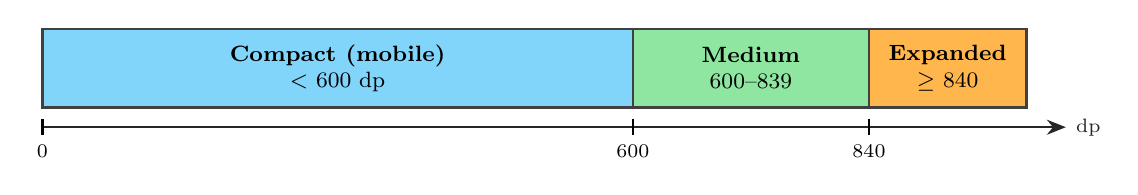
\begin{tikzpicture}
    \def\k{0.0125}
    \draw[base,fb,rounded corners=0pt] (0,0) rectangle (600*\k,1.0);
    \draw[base,fg,rounded corners=0pt] (600*\k,0) rectangle (840*\k,1.0);
    \draw[base,fo,rounded corners=0pt] (840*\k,0) rectangle (1000*\k,1.0);
    \node[font=\footnotesize,align=center] at (300*\k,0.5) {\textbf{Compact (mobile)}\\$<$ 600 dp};
    \node[font=\footnotesize,align=center] at (720*\k,0.5) {\textbf{Medium}\\600--839};
    \node[font=\footnotesize,align=center] at (920*\k,0.5) {\textbf{Expanded}\\$\geq$ 840};
    \draw[arr] (0,-0.25) -- (1000*\k+0.5,-0.25) node[right,font=\scriptsize]{dp};
    \foreach \v in {0,600,840}{\draw[thick] (\v*\k,-0.15) -- (\v*\k,-0.35); \node[font=\scriptsize,below] at (\v*\k,-0.35) {\v};}
  \end{tikzpicture}

  \vspace{6pt}
  \begin{columns}[T]
    \begin{column}{0.46\textwidth}
      \small
      \begin{itemize}\itemsep3pt
        \item \textbf{Breakpoint} là giá trị bề rộng (đơn vị \textbf{dp}) mà tại đó bố cục thay đổi.
        \item Dựa vào \textbf{bề rộng khả dụng}, không dựa vào tên thiết bị.
        \item Dùng \textbf{ít} breakpoint, đặt thành \textbf{hằng số} có tên.
        \item Mốc trên theo phân loại kích thước cửa sổ của \textbf{Material 3}.
      \end{itemize}
    \end{column}
    \begin{column}{0.52\textwidth}
\begin{lstlisting}[basicstyle=\ttfamily\fontsize{6.8}{8}\selectfont]
enum ScreenType { mobile, tablet }

class Breakpoints {
  static const double tablet = 600;

  static ScreenType fromWidth(double width) =>
      width >= tablet
          ? ScreenType.tablet
          : ScreenType.mobile;
}
\end{lstlisting}
    \end{column}
  \end{columns}
\end{frame}

\begin{frame}{1.2 Quy trình \textbf{chọn bố cục theo không gian khả dụng}}
  \centering
  \resizebox{0.97\linewidth}{!}{%
  \begin{tikzpicture}
    \node[dot] (s) at (0,0) {};
    \node[base,fb,minimum width=3.2cm] (lb) at (2.5,0) {\textbf{LayoutBuilder}\\nhận \textbf{constraints}};
    \node[base,fo,diamond,aspect=2.2,inner sep=1pt,minimum width=3.4cm] (d) at (7.0,0) {\textbf{maxWidth}\\$\geq$ breakpoint?};
    \node[base,fg,minimum width=3.4cm] (wide) at (11.8,1.3) {\textbf{Bố cục rộng}\\(nhiều vùng song song)};
    \node[base,fb,minimum width=3.4cm] (narrow) at (11.8,-1.3) {\textbf{Bố cục hẹp}\\(1 vùng, điều hướng)};
    \node[base,fg,minimum width=3.4cm] (out) at (11.8,-3.0) {\textbf{Build \& hiển thị}\\rebuild khi constraints đổi};
    \draw[arr] (s) -- (lb);
    \draw[arr] (lb) -- (d);
    \draw[arr] (d.east) |- node[lbl,above,pos=.75]{\textbf{đúng}} (wide.west);
    \draw[arr] (d.east) |- node[lbl,below,pos=.75]{\textbf{sai}} (narrow.west);
    \draw[arr] (wide.east) -- ++(0.7,0) |- (out.east);
    \draw[arr] (narrow.south) -- (out.north);
    \draw[darr] (out.west) -| node[lbl,pos=.2,above]{kéo / xoay} (lb.south);
  \end{tikzpicture}}
\end{frame}

\subsection{Nguyên tắc thiết kế cho nhiều màn hình và phương thức nhập liệu}

\begin{frame}{1.3 Nguyên tắc thiết kế giao diện thích ứng}
  \footnotesize
  \centering
  \begin{tikzpicture}
    \foreach \x/\y/\c/\t in {
      0/0/fb/{\textbf{1. Dựa vào không gian khả dụng}\\Đo bằng \textbf{LayoutBuilder}, không đoán loại thiết bị hay chỉ dựa hướng xoay.},
      4.7/0/fg/{\textbf{2. Giới hạn bề rộng nội dung}\\Dùng \textbf{max-width} để dòng chữ dễ đọc, form không bị giãn quá mức.},
      9.4/0/fo/{\textbf{3. Bảo toàn trạng thái}\\Đổi kích thước hoặc xoay \textbf{không làm mất} lựa chọn và dữ liệu đang xem.},
      0/-2.55/fg/{\textbf{4. Hỗ trợ đa phương thức nhập}\\\textbf{Chạm, chuột, bàn phím}: mỗi loại có cách tương tác phù hợp.},
      4.7/-2.55/fo/{\textbf{5. Trợ năng}\\Tôn trọng \textbf{cỡ chữ hệ thống}, theme sáng/tối, vùng chạm đủ lớn.},
      9.4/-2.55/fb/{\textbf{6. Không để tràn giao diện}\\Dùng Expanded / Flexible, cuộn nội dung; kiểm thử nhiều kích thước.}}{
      \node[base,\c,text width=3.9cm,minimum height=2.1cm,align=left,anchor=north west,inner sep=6pt] at (\x,\y) {\t};}
  \end{tikzpicture}
\end{frame}

\begin{frame}{1.3 Đa phương thức nhập liệu: \textbf{Touch}, \textbf{Mouse}, \textbf{Keyboard}}
  \footnotesize
  \renewcommand{\arraystretch}{1.5}
  \centering
  \begin{tabular}{@{}>{\raggedright\arraybackslash}p{2.2cm}>{\raggedright\arraybackslash}p{4.2cm}>{\raggedright\arraybackslash}p{6.0cm}@{}}
    \hline
    \rowcolor{cHead}\textbf{Phương thức} & \textbf{Đặc trưng} & \textbf{Cách thích ứng trong Flutter}\\ \hline
    \textbf{Touch} & Ngón tay, không có hover, cần vùng chạm lớn & Vùng chạm đủ lớn; cử chỉ \textbf{vuốt} (\api{Dismissible}), \api{GestureDetector}\\ \hline
    \textbf{Mouse} & Con trỏ chính xác, có \textbf{hover}, chuột phải & \api{InkWell}, \api{MouseRegion}, \api{mouseCursor}; nút bấm \textbf{hiển thị sẵn} thay cho cử chỉ ẩn\\ \hline
    \textbf{Keyboard} & Phím tắt, di chuyển bằng \textbf{focus} & \api{Shortcuts} / \api{Actions}, \api{CallbackShortcuts}, \api{Focus}\\ \hline
  \end{tabular}

  \vspace{8pt}
  \small \textbf{Nguyên tắc:} cùng một chức năng nên có \textbf{ít nhất một đường thao tác} phù hợp cho mỗi phương thức nhập.
\end{frame}

\begin{frame}{1.3 Tóm tắt phần cơ sở lý thuyết}
  \vspace{0.2cm}
  \begin{columns}[T]
    \begin{column}{0.32\textwidth}
      \begin{tikzpicture}
        \node[base,fb,text width=4.2cm,minimum height=3.7cm,align=left,anchor=north,font=\footnotesize,inner sep=7pt] {%
          \textbf{\normalsize Responsive / Adaptive}\\[3pt]
          $\bullet$ \textbf{Responsive}: co giãn liên tục\\
          $\bullet$ \textbf{Adaptive}: chọn bố cục riêng\\
          $\bullet$ Thực tế: \textbf{kết hợp} cả hai};
      \end{tikzpicture}
    \end{column}
    \begin{column}{0.32\textwidth}
      \begin{tikzpicture}
        \node[base,fg,text width=4.2cm,minimum height=3.7cm,align=left,anchor=north,font=\footnotesize,inner sep=7pt] {%
          \textbf{\normalsize Công cụ}\\[3pt]
          $\bullet$ \textbf{MediaQuery}: thông tin hệ thống\\
          $\bullet$ \textbf{LayoutBuilder}: đo vùng khả dụng\\
          $\bullet$ \textbf{Breakpoint}: ngưỡng đổi bố cục};
      \end{tikzpicture}
    \end{column}
    \begin{column}{0.32\textwidth}
      \begin{tikzpicture}
        \node[base,fo,text width=4.2cm,minimum height=3.7cm,align=left,anchor=north,font=\footnotesize,inner sep=7pt] {%
          \textbf{\normalsize Nguyên tắc}\\[3pt]
          $\bullet$ Dựa vào \textbf{không gian khả dụng}\\
          $\bullet$ \textbf{Max-width} cho nội dung\\
          $\bullet$ Hỗ trợ \textbf{touch, mouse, keyboard}\\
          $\bullet$ Bảo toàn \textbf{trạng thái}, trợ năng};
      \end{tikzpicture}
    \end{column}
  \end{columns}
\end{frame}

%% =====================================================================
%% PHẦN 2
%% =====================================================================
\section{Yêu cầu thực hành và demo}
\subsection{Tổng quan project Adaptive Notes}

\begin{frame}{2.1 \textbf{Adaptive Notes} -- ứng dụng ghi chú đa màn hình}
  \begin{columns}[T]
    \begin{column}{0.54\textwidth}
      \small
      \begin{itemize}\itemsep3pt
        \item Ứng dụng \textbf{ghi chú} Flutter minh hoạ \textbf{Responsive \& Adaptive UI}, \textbf{không dùng package bên ngoài}.
        \item \textbf{2 bố cục}: \textbf{Mobile} ($<$ 600 dp, 1 vùng) và \textbf{Tablet} ($\geq$ 600 dp, \textbf{Master--Detail}).
        \item Lưới thẻ chia \textbf{1 / 2 / 3 cột} theo bề rộng thực của vùng danh sách.
        \item \textbf{CRUD} đầy đủ: thêm, sửa, xoá (vuốt hoặc nút), \textbf{Hoàn tác} qua SnackBar.
        \item \textbf{Đa phương thức nhập}: chạm, chuột (hover), phím tắt \textbf{Ctrl+N}, \textbf{Ctrl+S}.
        \item Theme \textbf{sáng / tối}, cỡ chữ hệ thống, thanh \textbf{Layout Debug Bar}.
      \end{itemize}
    \end{column}
    \begin{column}{0.44\textwidth}
      \footnotesize
      \renewcommand{\arraystretch}{1.4}
      \begin{tabular}{@{}>{\raggedright\arraybackslash}p{1.9cm}>{\raggedright\arraybackslash}p{3.8cm}@{}}
        \hline
        \rowcolor{cHead}\textbf{Thành phần} & \textbf{Chi tiết}\\ \hline
        \textbf{Ngôn ngữ} & Dart\\ \hline
        \textbf{Framework} & Flutter, Material 3\\ \hline
        \textbf{Công cụ} & \api{LayoutBuilder}, \api{MediaQuery}, \api{Shortcuts}\\ \hline
        \textbf{Dữ liệu} & In-memory, 10 ghi chú mẫu\\ \hline
        \textbf{Kiểm thử} & \api{flutter\_test}\\ \hline
      \end{tabular}
    \end{column}
  \end{columns}
  \vspace{6pt}
  \small \textbf{GitHub:} {\bfseries\footnotesize\url{https://github.com/Duy-OC/Responsive-and-adaptive-UI}}
\end{frame}

\begin{frame}{2.1 Kiến trúc project (theo cấu trúc thư mục \texttt{lib/})}
  \centering
  \resizebox{!}{6.3cm}{%
  \begin{tikzpicture}
    \node[base,fo,minimum width=3.6cm] (main) at (0,4.2) {\textbf{main.dart}\\ThemeData sáng/tối, Material 3};
    \node[base,fb,minimum width=3.8cm] (home) at (0,2.6) {\textbf{HomeScreen}\\\textbf{LayoutBuilder} $\cdot$ State};
    \node[base,fb,minimum width=3.4cm] (edit) at (-5.2,2.6) {\textbf{NoteEditScreen}\\form $\cdot$ Ctrl+S};
    \node[base,fb,minimum width=3.4cm] (dscr) at (5.2,2.6) {\textbf{NoteDetailScreen}\\chi tiết (mobile)};
    \node[base,fg,minimum width=3.4cm] (mob) at (-4.0,1.0) {\textbf{MobileLayout}\\1 vùng};
    \node[base,fg,minimum width=3.4cm] (tab) at (1.0,1.0) {\textbf{TabletLayout}\\Row: flex 2 $\mid$ flex 3};
    \node[base,fg,minimum width=3.4cm] (list) at (-4.0,-0.6) {\textbf{NoteList}\\\textbf{LayoutBuilder} $\rightarrow$ cột};
    \node[base,fg,minimum width=3.0cm] (card) at (0,-0.6) {\textbf{NoteCard}\\hover $\cdot$ xoá};
    \node[base,fg,minimum width=3.4cm] (dview) at (5.0,-0.6) {\textbf{NoteDetailView}\\max-width 720 dp};
    \node[base,fo,minimum width=3.6cm] (help) at (-4.0,-2.3) {\textbf{responsive\_helper}\\gridColumns(), padding};
    \node[base,fo,minimum width=3.4cm] (bp) at (0.3,-2.3) {\textbf{Breakpoints}\\ScreenType, 600 / 900 dp};
    \node[base,fo,minimum width=3.0cm] (note) at (4.8,-2.3) {\textbf{Note} (model)\\bất biến};
    \draw[arr] (main) -- (home);
    \draw[darr] (home) -- (edit);
    \draw[darr] (home) -- (dscr);
    \draw[arr] (home) -- (mob);
    \draw[arr] (home) -- (tab);
    \draw[arr] (mob) -- (list);
    \draw[arr] (tab) -- (list);
    \draw[arr] (tab) -- (dview);
    \draw[arr] (dscr) -- (dview);
    \draw[arr] (list) -- (card);
    \draw[arr] (list) -- (help);
    \draw[arr] (help) -- (bp);
    \draw[arr] (card) -- (note);
  \end{tikzpicture}}
\end{frame}

\subsection{Bố cục thích ứng và minh hoạ mã nguồn}

\begin{frame}{2.2 Đáp ứng yêu cầu thực hành của project}
  \footnotesize
  \renewcommand{\arraystretch}{1.4}
  \centering
  \begin{tabular}{@{}>{\raggedright\arraybackslash}p{3.4cm}>{\raggedright\arraybackslash}p{9.0cm}@{}}
    \hline
    \rowcolor{cHead}\textbf{Yêu cầu} & \textbf{Cách project đáp ứng}\\ \hline
    \textbf{$\geq$ 2 kích thước / điều kiện hiển thị} & \textbf{Mobile} ($<$ 600 dp) và \textbf{Tablet} ($\geq$ 600 dp); lưới \textbf{1 / 2 / 3 cột}; xoay màn hình; cỡ chữ 1.0--2.0$\times$; sáng/tối\\ \hline
    \textbf{Chọn bố cục theo không gian khả dụng} & \api{HomeScreen}: \api{LayoutBuilder} đo \api{maxWidth} $\rightarrow$ \api{Breakpoints.fromWidth()}. \api{NoteList}: \api{LayoutBuilder} riêng đo \textbf{bề rộng vùng danh sách} $\rightarrow$ \api{gridColumns()}\\ \hline
    \textbf{Đa phương thức nhập liệu} & \textbf{Touch}: chạm, vuốt xoá. \textbf{Mouse}: hover, con trỏ \api{click}, nút xoá. \textbf{Keyboard}: \textbf{Ctrl+N}, \textbf{Ctrl+S}\\ \hline
    \textbf{Trợ năng \& chất lượng} & \api{MediaQuery.textScalerOf} co giãn chiều cao thẻ; \textbf{max-width} 640 / 720 dp; \textbf{Layout Debug Bar}; kiểm thử tự động\\ \hline
  \end{tabular}
\end{frame}

\begin{frame}{2.2 Sơ đồ quyết định bố cục trong project}
  \centering
  \resizebox{!}{6.2cm}{%
  \begin{tikzpicture}
    \node[dot] (s) at (-7.2,2.2) {};
    \node[base,fb,minimum width=3.2cm] (home) at (-5.2,2.2) {\textbf{HomeScreen}\\\textbf{LayoutBuilder}\\constraints.maxWidth};
    \node[base,fo,minimum width=3.2cm] (fw) at (-1.5,2.2) {\textbf{Breakpoints}\\\textbf{.fromWidth}(w)};
    \node[base,fo,diamond,aspect=2.2,inner sep=1pt,minimum width=2.8cm] (d1) at (2.4,2.2) {\textbf{w $\geq$ 600?}};
    \node[base,fg,minimum width=3.2cm] (tab) at (6.2,2.2) {\textbf{TabletLayout}\\Row: flex 2 $\mid$ flex 3};
    \node[base,fo,diamond,aspect=2.2,inner sep=1pt,minimum width=2.8cm] (d2) at (2.4,0.2) {\textbf{đang xem}\\\textbf{chi tiết?}};
    \node[base,fb,minimum width=3.2cm] (nds) at (-1.5,0.2) {\textbf{NoteDetailScreen}\\toàn màn hình};
    \node[base,fg,minimum width=3.2cm] (mob) at (6.2,0.2) {\textbf{MobileLayout}\\danh sách 1 vùng};
    \node[base,fb,minimum width=3.6cm] (nl) at (6.2,-1.8) {\textbf{NoteList}\\\textbf{LayoutBuilder} đo vùng};
    \node[base,fo,minimum width=3.4cm] (gc) at (1.6,-1.8) {\textbf{gridColumns}\\(w $-$ padding)};
    \node[base,fb,minimum width=2.9cm] (c1) at (-2.6,-3.7) {\textbf{1 cột}\\$<$ 400 dp};
    \node[base,fg,minimum width=2.9cm] (c2) at (1.6,-3.7) {\textbf{2 cột}\\400--899 dp};
    \node[base,fo,minimum width=2.9cm] (c3) at (5.8,-3.7) {\textbf{3 cột}\\$\geq$ 900 dp};
    \draw[arr] (s) -- (home);
    \draw[arr] (home) -- (fw);
    \draw[arr] (fw) -- (d1);
    \draw[arr] (d1) -- node[lbl,above]{\textbf{đúng}} (tab);
    \draw[arr] (d1) -- node[lbl,right]{\textbf{sai}} (d2);
    \draw[arr] (d2) -- node[lbl,above]{\textbf{có}} (nds);
    \draw[arr] (d2) -- node[lbl,above]{\textbf{không}} (mob);
    \draw[arr] (mob) -- (nl);
    \draw[arr] (tab.east) -- ++(0.6,0) |- (nl.east);
    \draw[arr] (nl) -- (gc);
    \draw[arr] (gc.south) -- ++(0,-0.4) -| (c1.north);
    \draw[arr] (gc.south) -- (c2.north);
    \draw[arr] (gc.south) -- ++(0,-0.4) -| (c3.north);
  \end{tikzpicture}}
\end{frame}

\begin{frame}{2.2 Minh hoạ bố cục theo không gian khả dụng}
  \centering
  \begin{tikzpicture}[
    fr0/.style={draw=black!75,thick,rounded corners=3pt,fill=white},
    bar/.style={fill=black!15,draw=black!60,thick},
    card/.style={draw=black!70,fill=cBlue,rounded corners=1.5pt,thick},
    det/.style={draw=black!70,fill=cGreen,rounded corners=1.5pt,thick}]
    % Mobile hẹp
    \draw[fr0] (0,0) rectangle (1.8,3.6);
    \draw[bar] (0,3.2) rectangle (1.8,3.6);
    \foreach \y in {2.45,1.7,0.95,0.2}{\draw[card] (0.15,\y) rectangle (1.65,\y+0.6);}
    \node[font=\scriptsize,align=center,text width=2.6cm] at (0.9,-0.65) {\textbf{Mobile hẹp}\\$<$ 400 dp nội dung\\\textbf{1 cột}};
    % Mobile rộng
    \draw[fr0] (3.0,0) rectangle (5.9,3.6);
    \draw[bar] (3.0,3.2) rectangle (5.9,3.6);
    \foreach \y in {2.45,1.7,0.95,0.2}{\draw[card] (3.15,\y) rectangle (4.4,\y+0.6); \draw[card] (4.5,\y) rectangle (5.75,\y+0.6);}
    \node[font=\scriptsize,align=center,text width=3.2cm] at (4.45,-0.65) {\textbf{Mobile rộng}\\400--599 dp\\\textbf{2 cột}};
    % Tablet
    \draw[fr0] (7.1,0) rectangle (13.6,3.6);
    \draw[bar] (7.1,3.2) rectangle (13.6,3.6);
    \foreach \y in {2.45,1.7,0.95,0.2}{\draw[card] (7.25,\y) rectangle (9.35,\y+0.6);}
    \draw[thick,black!70] (9.55,0) -- (9.55,3.2);
    \draw[det] (9.75,0.2) rectangle (13.45,3.05);
    \foreach \y in {2.6,2.2,1.8,1.4}{\draw[black!60,thick] (10.0,\y) -- (13.2,\y);}
    \node[font=\scriptsize] at (8.3,3.4) {flex 2};
    \node[font=\scriptsize] at (11.6,3.4) {flex 3};
    \node[font=\scriptsize,align=center,text width=6cm] at (10.35,-0.65) {\textbf{Tablet} $\geq$ 600 dp\\\textbf{Master--Detail}: danh sách $\mid$ chi tiết};
  \end{tikzpicture}
\end{frame}

\begin{frame}[fragile]{2.2 Code thực tế (1/3): chọn bố cục bằng \textbf{LayoutBuilder}}
  \begin{columns}[T]
    \begin{column}{0.60\textwidth}
\begin{lstlisting}[basicstyle=\ttfamily\fontsize{6.0}{7.0}\selectfont]
// breakpoints.dart
enum ScreenType { mobile, tablet }
static const double tablet = 600;
static ScreenType fromWidth(double width) =>
    width >= tablet ? ScreenType.tablet : ScreenType.mobile;

// home_screen.dart
Widget build(BuildContext context) => LayoutBuilder(
  builder: (context, constraints) {
    (*@\texttt{\itshape // Dựa vào không gian cha cấp, không suy đoán loại máy}@*)
    final type = Breakpoints.fromWidth(constraints.maxWidth);
    final detailVisible =
        type == ScreenType.mobile && _showDetail && ...;
    ...
    Expanded(
      child: type == ScreenType.tablet
          ? TabletLayout(notes: _notes, ...)
          : detailVisible
              ? NoteDetailScreen(note: selected, ...)
              : MobileLayout(notes: _notes, ...),
    ),
\end{lstlisting}
    \end{column}
    \begin{column}{0.38\textwidth}
      \footnotesize
      \begin{tikzpicture}
        \node[base,fb,text width=4.5cm,align=left,anchor=north] at (0,0) {\textbf{LayoutBuilder}\\Đo \api{maxWidth} của vùng cha cấp cho \api{HomeScreen}.};
        \node[base,fo,text width=4.5cm,align=left,anchor=north] at (0,-1.7) {\textbf{Breakpoint}\\\api{fromWidth()} đổi bề rộng thành \api{ScreenType} (ngưỡng \textbf{600 dp}).};
        \node[base,fg,text width=4.5cm,align=left,anchor=north] at (0,-3.6) {\textbf{Bảo toàn trạng thái}\\State (\api{\_notes}, \api{\_selectedId}) nằm \textbf{ngoài} LayoutBuilder nên đổi bố cục không mất dữ liệu.};
      \end{tikzpicture}
    \end{column}
  \end{columns}
\end{frame}

\begin{frame}[fragile]{2.2 Code thực tế (2/3): \textbf{Master--Detail} và lưới thích ứng}
  \begin{columns}[T]
    \begin{column}{0.60\textwidth}
\begin{lstlisting}[basicstyle=\ttfamily\fontsize{6.0}{7.0}\selectfont]
// tablet_layout.dart
Row(children: [
  Expanded(flex: 2, child: NoteList(...)),
  const VerticalDivider(width: 1),
  Expanded(flex: 3,
    child: selected == null
        ? const EmptyState(...)
        : NoteDetailView(note: selected!, ...)),
])

// responsive_helper.dart
int gridColumns(double availableWidth) {
  if (availableWidth >= Breakpoints.gridThreeColumns) return 3;
  if (availableWidth >= Breakpoints.gridTwoColumns) return 2;
  return 1;
}

(*@\texttt{\itshape // note\_list.dart: đo riêng vùng danh sách}@*)
LayoutBuilder(builder: (context, constraints) {
  final padding = horizontalPadding(constraints.maxWidth);
  final columns = gridColumns(constraints.maxWidth - padding * 2);
  return GridView.builder(
    gridDelegate: SliverGridDelegateWithFixedCrossAxisCount(
      crossAxisCount: columns, ...),
\end{lstlisting}
    \end{column}
    \begin{column}{0.38\textwidth}
      \footnotesize
      \begin{tikzpicture}
        \node[base,fg,text width=4.5cm,align=left,anchor=north] at (0,0) {\textbf{Adaptive}\\\api{Row} + \api{Expanded(flex: 2 / 3)} tạo bố cục \textbf{2 vùng} trên tablet.};
        \node[base,fb,text width=4.5cm,align=left,anchor=north] at (0,-1.7) {\textbf{Responsive}\\\api{gridColumns()} chia \textbf{1 / 2 / 3 cột} theo bề rộng nội dung (\textbf{400} và \textbf{900 dp}).};
        \node[base,fo,text width=4.5cm,align=left,anchor=north] at (0,-3.7) {\textbf{Đo đúng vùng}\\\api{NoteList} dùng LayoutBuilder \textbf{riêng} nên không phụ thuộc kích thước toàn màn hình.};
      \end{tikzpicture}
    \end{column}
  \end{columns}
\end{frame}

\begin{frame}[fragile]{2.2 Code thực tế (3/3): nhập liệu đa phương thức \& trợ năng}
  \begin{columns}[T]
    \begin{column}{0.60\textwidth}
\begin{lstlisting}[basicstyle=\ttfamily\fontsize{6.0}{7.0}\selectfont]
(*@\texttt{\itshape // home\_screen.dart: bàn phím}@*)
CallbackShortcuts(
  bindings: {
    const SingleActivator(LogicalKeyboardKey.keyN, control: true):
        () => _edit(),
  },
  child: Focus(autofocus: true, ...),
)

(*@\texttt{\itshape // note\_card.dart: chuột}@*)
InkWell(
  mouseCursor: SystemMouseCursors.click,
  onTap: onOpen, ...
)

(*@\texttt{\itshape // note\_list.dart: cảm ứng + cỡ chữ hệ thống}@*)
Dismissible(
  key: ValueKey(note.id),
  direction: DismissDirection.endToStart,
  onDismissed: (_) => onDelete(note), ...
)
(*@\texttt{\itshape // Chiều cao thẻ tăng theo cỡ chữ hệ thống}@*)
mainAxisExtent: 100 + scaler.scale(17) * 3 + ...,
(*@\texttt{\itshape // note\_detail\_view.dart: giới hạn bề rộng đọc}@*)
ConstrainedBox(
  constraints: const BoxConstraints(maxWidth: 720), ...)
\end{lstlisting}
    \end{column}
    \begin{column}{0.38\textwidth}
      \footnotesize
      \begin{tikzpicture}
        \node[base,fb,text width=4.5cm,align=left,anchor=north] at (0,0) {\textbf{Keyboard}\\\textbf{Ctrl+N} tạo ghi chú mới; \textbf{Ctrl+S} lưu trong màn hình sửa.};
        \node[base,fg,text width=4.5cm,align=left,anchor=north] at (0,-1.6) {\textbf{Mouse $\mid$ Touch}\\\api{InkWell} cho hover và con trỏ; \api{Dismissible} cho \textbf{vuốt xoá}.};
        \node[base,fo,text width=4.5cm,align=left,anchor=north] at (0,-3.2) {\textbf{Trợ năng}\\\api{textScaler} làm thẻ cao hơn khi chữ lớn, \textbf{max-width} giữ dòng chữ dễ đọc.};
      \end{tikzpicture}
    \end{column}
  \end{columns}
\end{frame}

\subsection{Kịch bản demo và kiểm thử}

\begin{frame}{2.3 Sơ đồ tuần tự: giao diện thích ứng khi đổi kích thước}
  \centering
  \renewcommand{\seqlen}{4.9}
  \resizebox{0.98\linewidth}{!}{%
  \begin{tikzpicture}
    \seqpart{u}{0}{fo}{\textbf{Người dùng}}
    \seqpart{h}{3.2}{fb}{\textbf{HomeScreen}\\(LayoutBuilder)}
    \seqpart{b}{6.4}{fo}{\textbf{Breakpoints}}
    \seqpart{n}{9.6}{fg}{\textbf{NoteList}\\(LayoutBuilder)}
    \seqpart{r}{12.8}{fo}{\textbf{responsive\_}\\\textbf{helper}}
    \smsg{0}{3.2}{-1.1}{kéo rộng cửa sổ / xoay}
    \smsg{3.2}{6.4}{-1.7}{\textbf{fromWidth}(maxWidth)}
    \sret{6.4}{3.2}{-2.3}{ScreenType.\textbf{tablet}}
    \smsg{3.2}{9.6}{-2.9}{build TabletLayout}
    \smsg{9.6}{12.8}{-3.5}{\textbf{gridColumns}(w)}
    \sret{12.8}{9.6}{-4.1}{1 / 2 / 3 cột}
    \sret{9.6}{0}{-4.65}{hiển thị lưới + chi tiết, \textbf{giữ} lựa chọn}
  \end{tikzpicture}}
\end{frame}

\begin{frame}{2.3 Kịch bản demo}
  \footnotesize
  \centering
  \begin{tikzpicture}
    \foreach \x/\y/\c/\t in {
      0/0/fb/{\textbf{1. Mobile dọc ($<$ 400 dp)}\\Danh sách \textbf{1 cột}; Layout Debug Bar hiển thị kích thước và loại bố cục.},
      7.0/0/fg/{\textbf{2. Xoay ngang / kéo rộng 400--599 dp}\\Lưới đổi sang \textbf{2 cột}, vẫn là bố cục Mobile.},
      0/-1.95/fo/{\textbf{3. Kéo rộng $\geq$ 600 dp}\\Chuyển sang \textbf{Master--Detail}: danh sách $\mid$ chi tiết.},
      7.0/-1.95/fb/{\textbf{4. Chọn ghi chú rồi đổi kích thước}\\Lựa chọn và dữ liệu được \textbf{giữ nguyên}.},
      0/-3.9/fg/{\textbf{5. Chuột \& bàn phím}\\Hover, \textbf{Ctrl+N}, \textbf{Ctrl+S}; vuốt trái để xoá rồi \textbf{Hoàn tác}.},
      7.0/-3.9/fo/{\textbf{6. Cỡ chữ lớn \& Dark mode}\\Tăng cỡ chữ hệ thống (đến 2.0$\times$): không tràn chữ.}}{
      \node[base,\c,text width=6.3cm,minimum height=1.6cm,align=left,anchor=north west,inner sep=6pt] at (\x,\y) {\t};}
  \end{tikzpicture}
\end{frame}

\begin{frame}{2.3 Kiểm thử tự động}
  \footnotesize
  \renewcommand{\arraystretch}{1.4}
  \centering
  \begin{tabular}{@{}>{\raggedright\arraybackslash}p{3.6cm}>{\raggedright\arraybackslash}p{8.9cm}@{}}
    \hline
    \rowcolor{cHead}\textbf{Tệp kiểm thử} & \textbf{Nội dung kiểm tra}\\ \hline
    \api{breakpoints\_test} & Đổi bố cục đúng tại \textbf{600 dp}; số cột tại 399 / 400 / 899 / 900; khoảng đệm theo bề rộng\\ \hline
    \api{note\_test} & Model \textbf{Note} bất biến; rút gọn xem trước 100 ký tự; dữ liệu mẫu độc lập\\ \hline
    \api{widget\_test} & Đổi kích thước \textbf{không mất lựa chọn}; thêm / sửa / xoá / hoàn tác; phím tắt; \textbf{không overflow} ở cỡ chữ 1.0--2.0$\times$, theme sáng và tối\\ \hline
    \api{check\_layout\_rules} & Công cụ kiểm tra tĩnh \textbf{12 quy tắc} thiết kế bố cục\\ \hline
  \end{tabular}
\end{frame}

%% =====================================================================
%% KẾT LUẬN
%% =====================================================================
\section{Kết luận}

\begin{frame}{3. Kết luận}
  \small
  \begin{itemize}\itemsep5pt
    \item \textbf{Responsive} co giãn bố cục liên tục; \textbf{Adaptive} chọn bố cục riêng theo điều kiện. Ứng dụng thực tế \textbf{kết hợp cả hai}.
    \item Nên dùng \textbf{LayoutBuilder} để chọn bố cục theo \textbf{không gian khả dụng}, dùng \textbf{MediaQuery} cho thông tin hệ thống (cỡ chữ, hướng, vùng an toàn).
    \item Đặt \textbf{breakpoint} thành hằng số, giới hạn \textbf{max-width} nội dung, bảo toàn \textbf{trạng thái} khi đổi kích thước.
    \item \textbf{Adaptive Notes} đáp ứng yêu cầu: \textbf{Mobile / Tablet}, lưới \textbf{1--3 cột}, hỗ trợ \textbf{touch, mouse, keyboard}, trợ năng và kiểm thử tự động.
  \end{itemize}
\end{frame}

\begin{frame}[plain]
  \centering
  \vspace{2.0cm}
  {\Huge\bfseries Xin cảm ơn\\[6pt] thầy và các bạn đã lắng nghe!}\\[16pt]
  {\Large\bfseries Hỏi \& Đáp}
\end{frame}

\end{document}
